\documentclass{article}


% if you need to pass options to natbib, use, e.g.:
%     \PassOptionsToPackage{numbers, compress}{natbib}
% before loading neurips_2022


% ready for submission
\usepackage[preprint]{neurips_2022}


% to compile a preprint version, e.g., for submission to arXiv, add add the
% [preprint] option:
%     \usepackage[preprint]{neurips_2022}


% to compile a camera-ready version, add the [final] option, e.g.:
%     \usepackage[final]{neurips_2022}


% to avoid loading the natbib package, add option nonatbib:
%    \usepackage[nonatbib]{neurips_2022}


\usepackage[utf8]{inputenc} % allow utf-8 input
\usepackage[T1]{fontenc}    % use 8-bit T1 fonts
\usepackage{hyperref}       % hyperlinks
\usepackage{url}            % simple URL typesetting
\usepackage{booktabs}       % professional-quality tables
\usepackage{amsfonts}       % blackboard math symbols
\usepackage{nicefrac}       % compact symbols for 1/2, etc.
\usepackage{microtype}      % microtypography
\usepackage{xcolor}         % colors
\usepackage{graphicx}       % graph
\usepackage{multirow}       % table multirow
\usepackage{algorithm, algorithmicx, algpseudocode}   % algorthim
\usepackage{threeparttable}
\usepackage{enumitem}
\usepackage{amssymb}
\usepackage{makecell}
\usepackage{wrapfig}	
\usepackage{bbding}
\usepackage{caption}
\usepackage{subfigure}
\bibliographystyle{plain}

\usepackage{amsthm,amsmath,amssymb}
\usepackage{mathrsfs}

\title{MSAT: Multi-stage adaptive threshold for Deep Spiking Neural Networks}


% The \author macro works with any number of authors. There are two commands
% used to separate the names and addresses of multiple authors: \And and \AND.
%
% Using \And between authors leaves it to LaTeX to determine where to break the
% lines. Using \AND forces a line break at that point. So, if LaTeX puts 3 of 4
% authors names on the first line, and the last on the second line, try using
% \AND instead of \And before the third author name.


\author{%
  David S.~Hippocampus\thanks{Use footnote for providing further information
    about author (webpage, alternative address)---\emph{not} for acknowledging
    funding agencies.} \\
  Department of Computer Science\\
  Cranberry-Lemon University\\
  Pittsburgh, PA 15213 \\
  \texttt{hippo@cs.cranberry-lemon.edu} \\
  % examples of more authors
  % \And
  % Coauthor \\
  % Affiliation \\
  % Address \\
  % \texttt{email} \\
  % \AND
  % Coauthor \\
  % Affiliation \\
  % Address \\
  % \texttt{email} \\
  % \And
  % Coauthor \\
  % Affiliation \\
  % Address \\
  % \texttt{email} \\
  % \And
  % Coauthor \\
  % Affiliation \\
  % Address \\
  % \texttt{email} \\
}


\begin{document}


\maketitle


\begin{abstract}
  Spiking Neural Networks(SNNs) can do inference with low-power consumption natively because of its spike sparsity.
  Compared with the other two traning method: STDP and BP, Conversion from Artifical Neural Networks(ANNs), is a more easlier way to acheive deep SNNs and commly have the approximate performance compared with ANN.
  However, Conversion SNNs suffer from a accuracy degration and more latency at inference time. Lots of studys have tryed to make a trade-off between improving accuracy and reduce the latency using varied method including adjust ANN topology
  when mapping ANN to SNN, using a more efficient fring mechanism et.al Here we analyze conversion loss layer-to-layer and point it out that membrane potential matters in both SNN accuracy and inference latency. 
  subsequently, we give a new perspective that most of current conversion method is optimization membrane potential to achieve higher accuracy and short latency.
  Meanwhile, Different from current converson schemes which use the same and invariant threshold with inference time in a layer, we propose a multi-stage adaptive threshold for deep spiking neural Networks.
  We examine the performance on CIFAR-100 and ImageNet for classfication. Futuremore, we show the propose method also behave well in objection detection on VOC and COCO. All above provide support  on biological interpretability.
\end{abstract}


\section{Introduction}

At present, Artificial Neural Network (ANN) is widely used in speech recognition, image processing and other fields.
However, with the complexity of neural
networks increasing progressively, running such deep networks
often requires large amounts of computational resources, such
as memory and power. In addition, current ANN's work mechanism differs from out brain. Actually, Neurons in the brain communicate by transmitting sequences (i.e. spike) generated by action potentials.  
Spiking Neuron network (SNN) works in a similar way. It also transmits the spike sequence to the downstream neurons. These spikes often carry a high amount of information, and the spike distribution is sparse, so it has the characteristics of low power consumption.  

SNNs potentially offer an efficient way of doing inference when it conbines with neuroncomputing hardware, futuremore, SNN inherently shows efficiency on processing temporal and spatial data. Its  
diverse coding mechanisms, and events-driven characteristics are also promising. However, because the internal state
variables of neurons do not satisfy the continuously differentiable
requirement, it is difficult to be trained. To solve this problem,
some algorithms based on the rules of gradient descent
and spike-time dependent plasticity (STDP) were proposed, which had partly solved the problem of training SNNs. 
Frustratingly, It is still difficult to train deeper SNNs with complex network 
structures, and results in a remaining of huge gap of
performance between SNNs and CNNs in complex recognition or detection tasks.

To narrow the performance gap between SNNs and CNNs, methods of converting CNNs to SNNs had been proposed. 
In these methods, a CNN is firstly trained using the standard stochastic gradient
descent and back propagation algorithm, and then the trained
weights are mapped to an SNN with the same structure as the
CNN. Inference is performed on the converted SNNs. The main idea is that the firing rates of spiking neurons can approximate the
activations of their counterparts (RELU) in ANNs  with sufficient time
steps. This finding has become the fundamental principle
underlying the conversion scheme. Converted SNNs often suffer from a accu-
racy degration and more latency at inference time. Lots of studys have tryed to
make a trade-off between improving accuracy and reduce the latency using var-
ied method including adjust ANN topology when mapping ANN to SNN, using
a more efficient fring mechanism et.al. Here we forms conversion loss formula and shows that residual membrane potential in each IF neuron 
increase the latency which mean firing rates approximate to activation value. We also find that most of current converson schemes,
they use threshold invariant with inference time and are same and in a layer. This mechanism is inconsistent with a phenomenon which has been widely observed in 
the central nervous system, e.g. visual cortex , auditory 
midbrain, hippocampus, somatosensory cortex.  It has 
been proposed that threshold variability reflects 
an adaptation of the spike threshold to the membrane potential. Inspired by this, we propose a multi-stage adaptive threshold for deep spiking neural Networks. 
For each neuron, its threshold vaires with its own membrane potential.We both do experimental on object recognition and detection in non-trival datasets to prove
proposed method is as well as efficiency with the current mainstream schemes when doing visual tasks.

Our major contribution can be summarized as:
\begin{itemize}
  \item sufficient experimental on object recognition and detection in non-trival datasets, shows that our proposed method is both efficiency and biological interpretability
  \item a formula on layer-by-layer conversion error, a new perspective diving existing method into three part 
  \item a multi-stage adaptive threshold mechanism, which is widely existing in the center nervous system and thus more biological plausible. We use it for deep spiking neural Networks.
\end{itemize}


\section{PRELIMINARIES}
Our conversion pipeline exploits the threshold balancing mechanism (Diehl et al., 2015; Sengupta
et al., 2018) between ANN and SNN with modified ReLU function on the source ANN to reduce
the consequential conversion error. Through in this mechanism, we give a two-layer MLP conversion Framework 
Diagram as fig1 to Convenient for our discussion.

\begin{figure}[htbp]
  \centering
  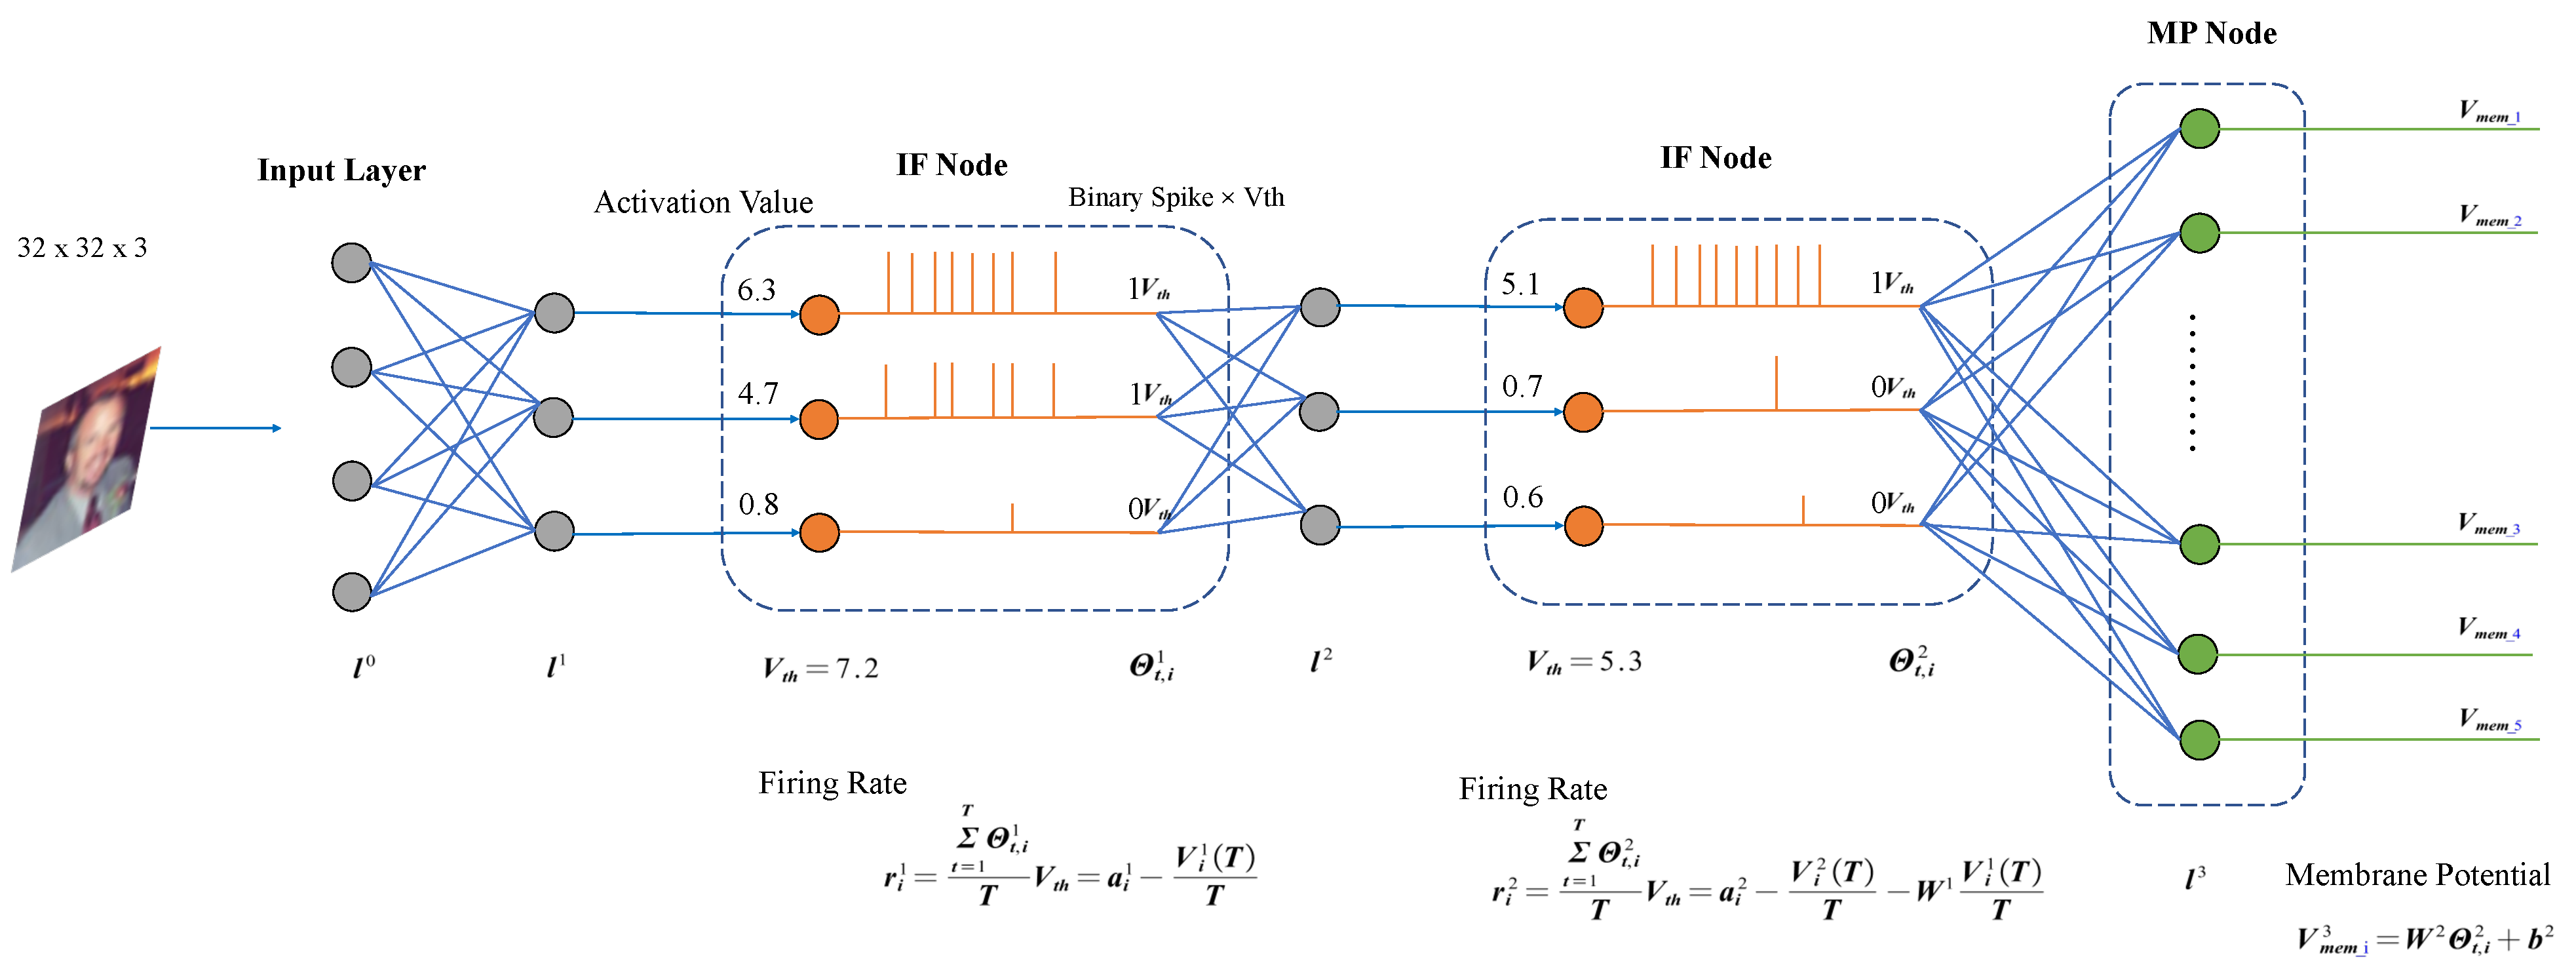
\includegraphics[width=0.95\textwidth]{t.pdf}
  \caption{A two-layer MLP conversion Framework for demonstration.}
\end{figure}

The main idea in ANN-to-SNN conversion is using mean firing rate $r_i^l(t)$ which indicates firing rate of neuron $i$ in layer $l$ for a total time t to approximate the activation value $a_i^l$ in SNN.
Here we give analytical explanation for the approximation.

In ANN, the neuron i activation value(after relu) in layer l $a_i^l$ can be computed as:
\begin{equation}
  a_i^l = max\left(0, \sum_{j=1}^{M^{l-1}}W_{ij}^la_j^{l-1} + b_i^l\right)
\end{equation}
here $l \in \{1, \cdots ,L\}$ indicates layer $l$ in a network with L layers; $W_{ij}^l$ indicates weight connection between neuron $i$ in layer $l$ and neuron $j$ in layer $l-1$;
$b_i^l$ indicates neuron $i$ bias in layer $l$; it is worth noting that $a_i^l$ start from $l=0$ and $a^0=x$.


\paragraph{Neuron Model} postsynaptic membrane potential(PSP) at timestep $t+1$, $V_i^l(t+1)$ is a sum of last timestep membrane potential and current input electric current. When PSP exceeds a certain voltage threshold, it emits an output spike and reset the membrane potential.
One of the most widely adopted model is Integrate-and-Fire (IF) neuron, and membrane potential at the next time
step t + 1 would then be updated by soft-reset mechanism, which subtract threshold in PSP rather than reset the membrane potential to $V_{reset}$. The mathematical form is as follows.
\begin{equation}
V_i^l(t + 1)=V_{i}^{l}(t)+V_{th}^l\left(\sum_j^{M^{l-1}}W_{ij}^l\Theta_{t,j}^{l-1}+b_i^l\right)-V_{th}^l\Theta_{t,i}^{l}
\end{equation}

here $\Theta_{t,i}^{l}$ is a function indicating the neuron $i$ in layer $l$ occurrence of a spike at time $t$
\begin{equation}
  \Theta_{t, i}^{l}=\Theta\left(V_{i}^{l}(t-1)+z_{i}^{l}(t)-V_{th}^l\right), with \; \Theta(x)= \begin{cases}1 & \text { if } x \geq 0 \\ 0 & \text { else }\end{cases}
\end{equation}
Here $z_i^l(t)$ is neuron $i$ inputs in layer $l$ and time $t$
\begin{equation}
  z_{i}^{l}(t) = V_{th}^l\left(\sum_j^{M^{l-1}}W_{ij}^l\Theta_{t,i}^{l}+b_i^l\right)
\end{equation}

\section{Diving Conversion Error}
Error comes from two part: one is converting ANN to SNN directly, result quantization error and clip error; the other is spike arrtribute, result residual potential error.
show as fig 2
\begin{figure}[htbp]
  \centering
  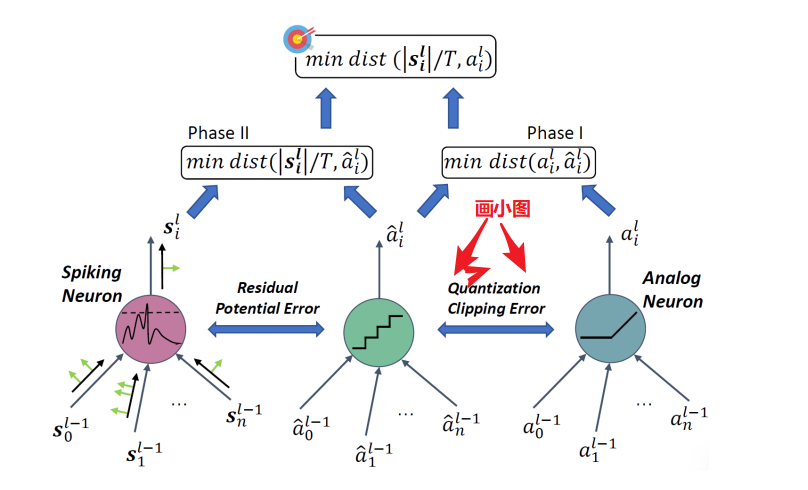
\includegraphics[width=0.95\textwidth]{test.png}
  \caption{Three error.}
\end{figure}
\subsection{Layer-By-Layer Quantization Error}

For equation (2), cumulate the input over the simulation timestep T, we can derive the firing rate relationship layer-to-layer.
\begin{equation}
  V_{th}^l\sum_{t=0}^T\Theta_{t,i}^{l}=\sum_{t=0}^TV_{th}^l\left(\sum_j^{M^{l-1}}W_{ij}^l\Theta_{t,j}^{l-1}+b_i^l\right) - V_i^l(T)
\end{equation}


\begin{equation}
  r_i^l(T) = \sum_j^{M^{l-1}}W_{ij}^lr_j^{l-1}+b_i^l - \frac{V_i^l(T)}{TV_{th}^{l}}
\end{equation}

Unfolding for each layer, relationship between mean fring rate and activation value can be shown as following:
\begin{equation}
  \begin{aligned}
    r_i^l(T) &=\sum_j^{M^{l-1}}W_{ij}^lr_j^{l-1}+b_i^l - \frac{V_i^l(T)}{TV_{th}^{l}} \\
    &=\sum_j^{l-1} \sum_j^{M^{l-1}}W_{ij}^l\left(\sum_k^{M^{l-2}}W_{jk}^{l-1}r_k^{l-2}+b_j^{l-1} - \frac{V_j^{l-1}(T)}{TV_{th}^{l-1}} \right) + b_i^l - \frac{V_i^{l}(T)}{TV_{th}^{l}}\\
    &= \begin{split}
        &\sum_j^{l-1} \sum_j^{M^{l-1}}W_{ij}^l\left(\sum_k^{M^{l-2}}W_{jk}^{l-1}\left(\sum\cdots \underbrace{\sum_m^{M^{1}}W_{1m}^1x_m+b_m^1}_{a_m^1} - \frac{V_i^1(T)}{TV_{th}^{1}} + \cdots + b - \frac{V(T)}{TV_{th}} \right) \right.\\ 
        &\left. + b_j^{l-1} - \frac{V_j^{l-1}(T)}{TV_{th}^{l-1}} \right) + b_i^l - \frac{V_i^{l}(T)}{TV_{th}^l}
    \end{split}
\end{aligned}
\end{equation}

Use $\Delta V_i^l$ denotes $\frac{V_i^{l}(T)}{TV_{th}^l}$

则上面的式子变为
\begin{equation}
    r_i^l(T) = a_i^l - \Delta V_i^l - \sum_j^{M^{l-1}}W_{ij}\Delta V_j^l - \cdots -\sum_j^{M^{l-1}}W_{ij}^l \cdots \sum_k^{M^{1}}W_{1k}^2 \Delta V_k^1
\end{equation}

Note that the activation value is strictly fall in [0, 1] by using weight normalization.
So the weights are not origin ANN weight and are scaled by $V_{th}^{l-1}/V_{th}^l$ and bias are scaled by $V_{th}^l$ and $V_{th}$ is set to 1.
It has the same form with threshold balancing, the different is that threshold balancing use postsynaptic neuron threshold times firing spike to compute mean firing rate
Actually, Two method: weight normalization and threshold balancing are mathematically equivalent. We use threshold balancing in rest of paper for convenience.

Bias is a constant all the time so it does't affect the conversion error and we omit it and in threshold balancing, mean firing rate $r_i^l(t)$ is PSP average value, so equation (5) becomes
\begin{equation}
  r_i^l(T) = \sum_j^{M^{l-1}}W_{ij}^lr_j^{l-1} - \frac{V_i^l(T)}{T}
\end{equation}

When $V_{th}^l$ is larger than maximum of activation value, $V_i^l(T)$ will be less than $V_{th}$ thus the residual membrane potential cannot be output thats why information transmition suffer a loss.
There error is basically because the discrete of timestep that the mean firing rate is a step function which cannot exactly approximate the source continuous RELU function, which is known as quantization error (flooring error), is can be expressed as
\begin{equation}
  r_i^l(T) = \operatorname{clip}\left(\frac{V_{th}^l}{T}\left\lfloor\frac{W_{ij}^lr_j^{l-1}T}{V_{th}^l}\right\rfloor, 0, V_{th}\right)
\end{equation}

\subsection{Maximum Activation Clip Error}
As mentioned in equation (9), if voltage threshold is set less than maximum activation value, then when PSP exceeds voltage threshold, the emited spike will not transmit efficient information to distinct above PSP.
Set voltage threshold to maximum activation value can avoid this but suffer a huge latency. This is a trade-off, and in (Sengupta), choose quantile p for different datasets. (Li ) propose a Bayesian Optimization to find this p value.
\begin{equation}
  r_i^l(T) = \sum_j^{M^{l-1}}W_{ij}^lr_j^{l-1} - \frac{a_{max}^l-V_{th}^l}{T}
\end{equation}

\subsection{Spike inherently Error}
This is unavoidable in early timestep, mainly caused by iiregular arrving spike. The phenomenon is that the suddenly coming spike or inactivation neuron wrong spike.
\begin{figure}[htbp]
  \centering
  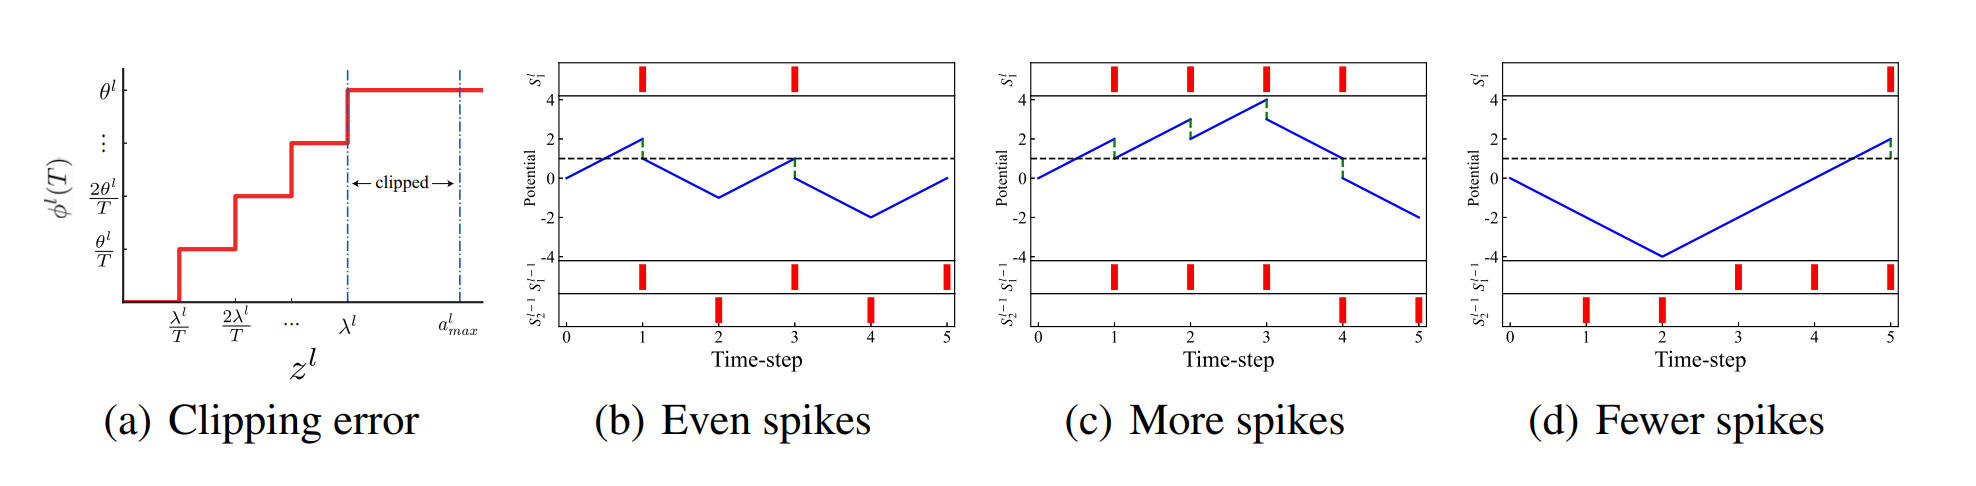
\includegraphics[width=0.95\textwidth]{test2.png}
  \caption{Spike inherently Error}
\end{figure}

Larger timestep or spike calibration can relieve this error while cannot eliminate it. 

\section{Method}
\subsection{adaptive threshold still holds}
Let's take a look at existing methods, no matter weight normalization or threshold balancing, they aim at zipping the gap between ANN and SNN. Though, we should be aware that
the real advantage of SNN is its sparse spike which simultaneously low-power and brain-Inspired. Current method, however, set threshold voltage as the same in the same layer and 
these threshold will remain unchanged despite inference time increasing. It ignores a fact that neurons in different
regions of brain represent distinct dynamics and process information differently from other regions. 
The threshold voltage of neurons is also known to have a broad
range rather than a single value. Some neuronscience literature indicates that threshold value 
is variable in the same neuron and threshold 
variability is a genuine feature of neurons, which reflects 
adaptation to the membrane potential at a short 
timescale. Thus the voltage threshold should different from neurons and timestep. Here we demonstrate that voltage threshold is a function of timestep t and the transmits the equivalent information with the constant threshold.

obmitting the bias, the equation(5) can be rewrited as the following form
\begin{equation}
  V_i^l(t)=V_{i}^{l}(t-1)+\sum_j^{M^{l-1}}V_{th,j}^l(t)W_{ij}^l\Theta_{t,j}^{l-1}+b_i^l -V_{th,i}^l(t)\Theta_{t,i}^{l}
\end{equation}

firing rate during timestep T is computed as 
\begin{equation}
  r_i^l(T) = \frac{\sum_{t'=1}^{T}V_{th,i}^l(t')\Theta_{t',i}^{l}}{T}
\end{equation}

the firing rate relationship in higher layer, it means equation (9) still satisfy so the conversion error form is the same.
But note that the residual neuron membrane potential $V_i(T)$ can be faster adjusted, so the spike information could be more efficiency and thus shorten the conversion latency. 

Above equation ensures that all the output neurons are used and adjust the neurons' thresholds to the stimuli for which they become specialized. 

\subsection{Multi-stage adaptive threshold}

In vivo, the spiking threshold displays large variability. This phenomenon has been widely observed in
the central nervous system, e.g. visual cortex \cite{azouz2000dynamic, azouz2003adaptive}, auditory
midbrain \cite{pena2002postsynaptic}, hippocampus \cite{henze2001action}, somatosensory cortex \cite{wilent2005stimulus}. It has
been proposed that threshold variability measured in vivo reflects
an adaptation of the spike threshold to the membrane potential. To our best knowledge, threshold varies in conversion is fewly used in \cite{kim2020towards,chen2022adaptive,li2021free} whild they only use two-stage or heuristic method and still cannot represent the homoeostasis well.

Inspired by this, we propose a adaptive threshold, which is multi-stage and vaires with inference time.
The method can be briefly sumed up as: \textbf{varies with firing history and input properties},
Specifically, spike threshold is positively correlated with the average $V_i$ preceding spikes and negatively correlated with the rate of depolarization. Also, it is consistent with some
other threshold adaptation models: the threshold increases after each spike and decreases if there is no spike.
The relationship between threshold and membrane potential and rate of depolarization is described as
\begin{equation}
  V_{th}(t+1) = \tau_{mp}V_{th\_mp}(t) + \tau_{rd}V_{th\_rd}(t+1)
\end{equation}

Where $\tau_{mp}$ and $\tau_{rd}$ is the time constant of the dynamic tracking threshold $V_{th\_mp}(t)$ and dynamic evoked threshold $V_{th\_rd}(t+1)$ separately.

\paragraph{dynamic tracking threshold(DTT)} DTT is a flection of spiking threshold vaires with firing history. It shows that spike threshold depends on preceding membrane potential
and tracking the membrane potential at a short timescale due to inactivation of sodium channel\cite{kuba2010presynaptic, hu2009distinct, platkiewicz2011impact} or the activation of potassium channels\cite{higgs2011kv1, goldberg2008k}.
in \cite{fontaine2014spike}, the DTT is a similar first-order kinetic equation, we here use steady-state threshold for fitting our SNNs.
we use $V_{m,i}^l(t)$ to denote the average membrane potential during timestep $t$ in layer $l$ neuron $i$, then DTT is following:
\begin{equation}
  V_{th\_mp}^l(t) = \left(\alpha\left(V_i^l(t)-V_m^l(t)\right)+V_{T}^l+k_aln\left(1+e^{\frac{V_i^l(t)-V_m^l(t)}{k_i}}\right)\right)
\end{equation}

here $\eta, k$is both time constant, $V_{T}^l$ is the parameters to optimize. when PSP is less than average membrane potential $V_m^l(t)$, the slope is $\eta$ on the left side of the knee. The slope on the right side is $\frac{k_a}{k_i} + \alpha$. The curvature C is determined by $\alpha, k_a, k_i, V_{T}^l, V_i^l(t)$.

idealy, when spike reaches to stabality, the $V_i^l(t) \to V_m^l(t)$ so DTT term will be very small.
the threshold increas with membrane potential and thus any voltage fluctuations that are slower than threshold adaptation should not have an impact on output spiking, this is indirectly relieve the spike inherently error.

\paragraph{dynamic evoked threshold(DET)} DET is a flection of spiking threshold vaires with input properties. paper

\begin{equation}
  V_{th\_rd}^l(t+1) = \tau_{rd}\left(e^{-\mid\mu\left(V_i^l(t)\right)\mid} + e^{-\frac{\left(V_i^l(t+1)-V_i^l(t)\right)}{C}}\right)
\end{equation}

idealy, when spike reaches to stabality, the $V_i^l(t+1) \to V_i^l(t)$ so DET term will be very small.

\paragraph{Interaction of DET and DTT} Take together, the causal link between preceding spike membrane potential and neg-
atively correlated with the rate of depolarization, shows that threshold adaptation neurons selective to fast input variations and remarkably insensitive to slow ones. In other words, the slow voltage fluctuations are filtered out by threshold adaptation.

Thus our adaptive threshold can be formed as:
\begin{equation}
  V_{th,i}^l(t+1) = \tau_{mp}\left(\eta\left(V_i^l(t)-V_m^l(t)\right)+ln\left(1+e^{\frac{V_i^l(t)-V_m^l(t)}{\psi}}\right)\right) + \tau_{rd}\left(e^{-\mid\mu\left(V_i^l(t)\right)\mid} + e^{-\frac{\left(V_i^l(t+1)-V_i^l(t)\right)}{C}}\right)
\end{equation}

Above equation ensures that all the output neurons are used and adjust the neurons’ thresholds to the
stimuli for which they become specialized.
The pseudocodes for adaptive threshold algorithm are shown in Algorithm 1.
\begin{algorithm}[h] 
	\caption{Conversion from ANN to SNN: Multi-stage adaptive threshold(\# todo)} 
	\begin{algorithmic}[1] 
		\Require 
    Pretrained ANN, training set,  SNN's inference timestep T
		\Ensure 
		The converted SNN firing rate approximate ANN activation value with shorter latency

    \For {s = 1 to \# of samples}
      \State $a_l \gets$ layer-wise activation value
      \For {$l$ = 1 to L}
        \State $V_{th}^l \gets \frac{1}{2}max[V_{th}^l, max(a_l)]$
        \State $SNN.layer[l].V_{th} \gets V_{th}^l$
      \EndFor
    \EndFor

    \For {t = 1 to timestep T}
      \For {$l$ = 1 to L}
        \For{$j$ = 1 to neuron number of layer $l$}
          \State $dV_{th} \gets \gamma(SNN.layer[l].R[j] - SNN.layer[l].V_{mem}[j])$
          \State $SNN.layer[l].V_{th}[j] \gets SNN.layer[l].V_{th}[j] + dV_{th}$
        \EndFor
      \EndFor
    \EndFor

	\end{algorithmic} 
\end{algorithm}




\section{EXPERIMENTS}


Extensive experiments 

\begin{table}[!t]
  \centering
  \caption{Experimental results on CIFAR100}
  \begin{threeparttable}
    \resizebox{\linewidth}{!}{
      \begin{tabular}{c|c|c|ccccc}
        \toprule
        Method& Use DT &ANN &SNN Best & T=32 & T=64 & T=128 & T=256\\
        \midrule
        \multicolumn{8}{c}{\textbf{VGG16, CIFAR100}}\\
        \midrule
        p-Norm \cite{rueckauer2017conversion} &\XSolid & 78.49& 58.44 & 44.88 & 51.89 & 56.02 & 58.44 \\
        Channel-Norm\cite{kim2020spiking} &\XSolid & 78.49 & 74.74 & 54.03 & 67.34 & 72.50 & 74.73 \\
        Spike-Norm\cite{sengupta2019going} &\XSolid& 71.22 & 70.77& - & - & - & -\\
        TSC\cite{han2020deep} &\XSolid &71.22 & 70.97 &- &- & 69.86 & 70.65 \\
        RMP-SNN\cite{han2020rmp} &\XSolid&71.22 & 70.93 &- &- &63.76 & 68.34\\
        Opt.\cite{deng2021optimal} &\XSolid& 77.89& 77.71 & 7.64 & 21.84 & 55.04 & 73.54\\
        Calibration\cite{li2021free} &\XSolid& 77.89 & 77.87 & 73.55 & 76.64 & 77.40 & 77.68\\
        Burst \cite{li2022efficient} &\XSolid& 78.49 & 78.71 & 74.98 & 78.26 & 78.66 & 78.65 \\
        \textbf{This Work} &\Checkmark&78.49 & \textbf{78.64} & \textbf{63.26} & \textbf{75.46} & \textbf{78.13} & \textbf{78.58} \\
        \midrule
        \multicolumn{8}{c}{\textbf{ResNet20, CIFAR100}}\\
        \midrule
        p-Norm \cite{rueckauer2017conversion} &\XSolid& 80.69& 67.35 & 38.13 & 58.09 & 64.96 & 67.33  \\
        Channel-Norm\cite{kim2020spiking} &\XSolid& 80.69 & 71.26 & 52.59 & 66.05 & 70.08 & 71.26\\
        Spike-Norm\cite{sengupta2019going}&\XSolid & 68.72 & 64.09& - & - & - & - \\
        TSC\cite{han2020deep} &\XSolid &68.72 & 68.18 &- &- & 58.42 & 65.27 \\
        RMP-SNN\cite{han2020rmp} &\XSolid&68.72 &67.82  &27.64 &46.91 &57.69 & 64.06\\
        Opt.\cite{deng2021optimal} &\XSolid& 77.16& 77.22 & 51.27 & 70.12 & 75.81 & 77.22\\
        Calibration\cite{li2021free} &\XSolid& 77.16 & 77.73 & 76.32 & 77.29 & 77.73 & 77.63\\
        Burst \cite{li2022efficient}  &\XSolid& 80.69& 80.72 & 76.39 & 79.83 & 80.52 & 80.57   \\
        \textbf{This Work } &\Checkmark&80.69 & \textbf{80.58} & \textbf{71.98} & \textbf{78.58} & \textbf{80.25} & \textbf{80.57}\\
        \bottomrule
    \end{tabular}}
  \end{threeparttable}
  \label{cifar100}
\end{table}

\begin{table}[!t]
  \centering
  \caption{Summary of given hyperparameters on different network}
  \setlength{\tabcolsep}{9mm}{
      \begin{tabular}{c | c | c}
        \toprule
        Symbol& VGG16 &ResNet20 \\
        \midrule
        $\alpha$ & 0.03 & 0.3 \\
        $k_a$ & 1 & 1\\
        $k_i$ & 1.0 & 1.0\\
        $C$ & 5.0 & 5.0 \\
        $\tau_{mp}$ & 1 & 0.5\\
        $\tau_{rd}$ & 1 & 0.5\\
        \bottomrule
    \end{tabular}}
  \label{hyperparameters}
\end{table}




\begin{figure}[htbp]
  \centering
  \subfigure[pic1.]{
  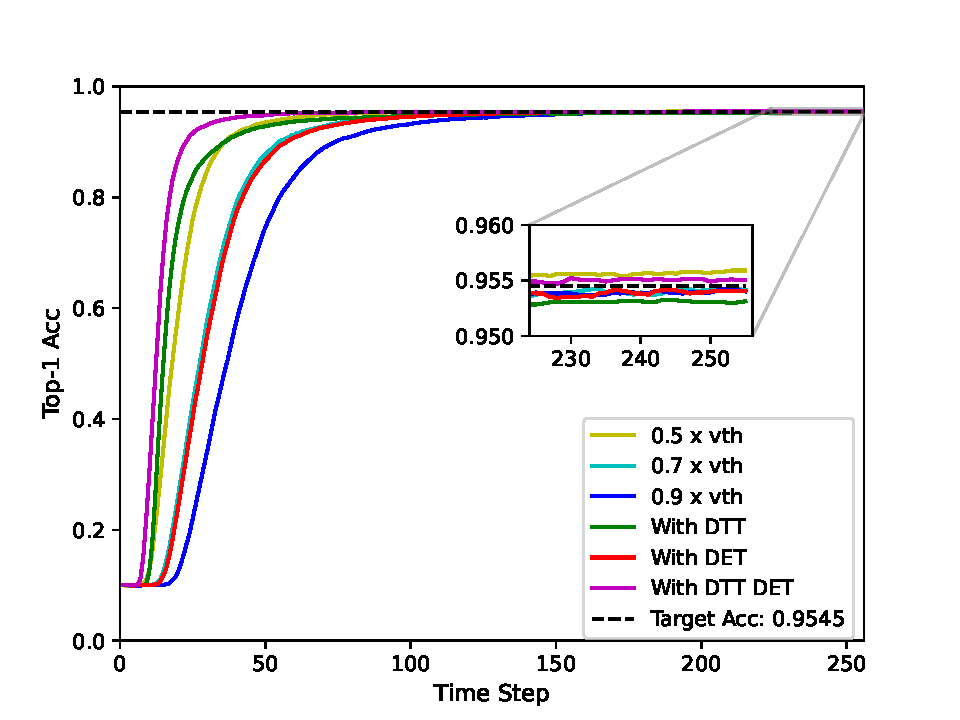
\includegraphics[width=6cm]{./fig/acc_cifar10_vgg16.pdf}
  %\caption{fig1}
  }
  \quad
  \subfigure[pic2.]{
  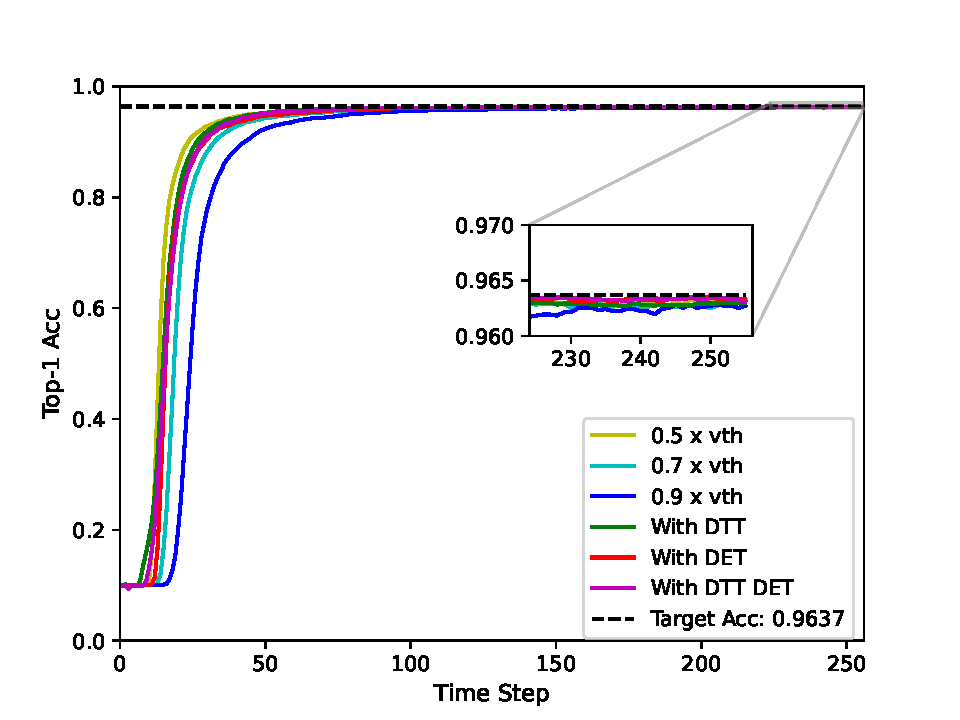
\includegraphics[width=6cm]{./fig/acc_cifar10_resnet20.pdf}
  }

  \subfigure[pic3.]{
    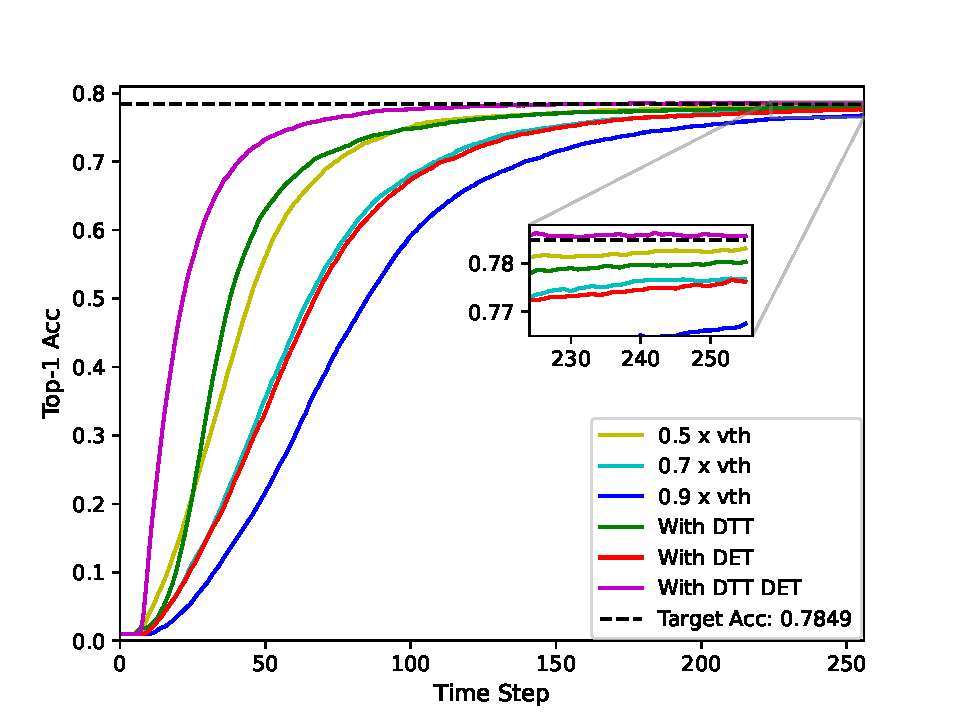
\includegraphics[width=6cm]{./fig/acc_cifar100_vgg16.pdf}
    %\caption{fig1}
    }
    \quad
    \subfigure[pic4.]{
    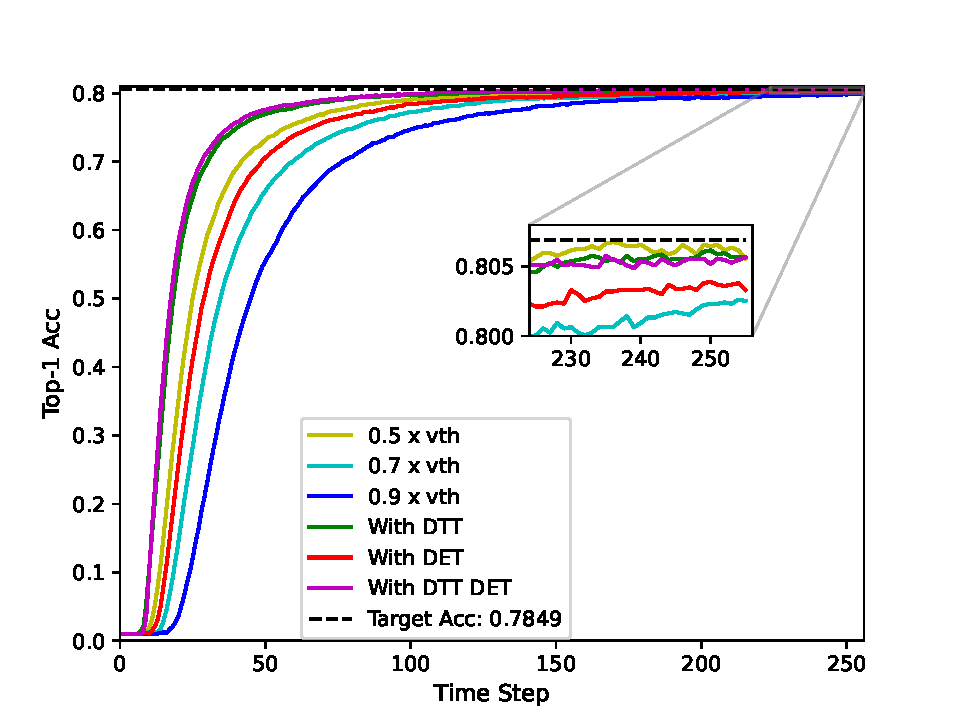
\includegraphics[width=6cm]{./fig/acc_cifar100_resnet20.pdf}
    }

  \caption{ pics}
  \end{figure}

\begin{figure}[h]
  \centering
  \fbox{\rule[-.5cm]{0cm}{4cm} \rule[-.5cm]{4cm}{0cm}}
  \caption{Spike count(efficiency) fig.}
\end{figure}




Table x: detection mAP on VOC and COCO for our converted SNNs, and compared to other conversion methods and ANN.


\begin{figure}[htbp]
  \centering
  \fbox{\rule[-.5cm]{0cm}{4cm} \rule[-.5cm]{4cm}{0cm}}
  \caption{Vth vaires result vs inherent inference timestep.}
\end{figure}

\section{discussion}

Indeed a trivial solution to
the fitting problem is the threshold model defined by  and th~0 ms: the ‘‘spike threshold’’ always equals
the membrane potential, in particular at the upstroke of spikes.
To avoid these problems, we instead used the threshold model
to predict the occurrence of spikes and their precise timing based
only on Vm. The trivial solution mentioned above is a poor
predictor of spikes since it would predict too many spikes

%%%%%%%%%%%%%%%%%%%%%%%%%%%%%%%%%%%%%%%%%%%%%%%%%%%%%%%%%%%%%%%
\newpage
\bibliography{neurips_2022}

%%%%%%%%%%%%%%%%%%%%%%%%%%%%%%%%%%%%%%%%%%%%%%%%%%%%%%%%%%%%


\appendix


\section{Appendix}


Optionally include extra information (complete proofs, additional experiments and plots) in the appendix.
This section will often be part of the supplemental material.


\end{document}